\documentclass[portuguese,oneside]{tcc}

\usepackage{graphicx}
\usepackage{multirow}
\usepackage{nicefrac}
\usepackage{algorithmic}
\usepackage{calc}
\usepackage{enumitem}
\usepackage{fixltx2e}

\author{Guilherme de Mello Mattos Taschetto e Pedro Pillon Vanzella}

\title{Inteligência Artificial Aplicada a Elevadores}
      {Artificial Intelligence Applied to Elevators}

\tipotrabalho{\tci}
\curso{\cc}
\orientador{João Batista de Oliveira}

\begin{document}

\begin{resumo}{elevadores, inteligência artificial, simulação, sistemas multiagentes, aprendizado de máquina}

Elevadores são um meio de transporte utilizado por milhões de pessoas no mundo
inteiro. Com este trabalho, pretende-se propor soluções de Inteligência
Artificial para melhorar a eficiência dos mesmos, reduzindo o tempo que
passageiros despendem em função destes. Através da modelagem e implementação de
um simulador de elevadores e de algoritmos de Inteligência Artificial, espera-se
realizar testes de diferentes técnicas e soluções propostas na literatura, a fim
de propor quais estratégias são mais adequadas para cada cenário.

\end{resumo}

\begin{abstract}{elevators, artificial intelligence, simulation, multiagent systems, machine learning}

Elevators are a mode of transportation used by milions of people around the
world. In this project, we will propose Artificial Intelligence solutions in
order to increase their efficiency, reducing their users' wait times. Through
the process of modeling and implementation of an elevator simulator and
Artificial Intelligence algorithms, we hope to test out the different techniques
and solutions proposed in the literature, in order to propose which strategies
best fit each scenario.

\end{abstract}

\tableofcontents

\chapter{\label{chap:intro}Introdução}

Em 2014, 54\% da população mundial vivia em áreas urbanas, de acordo com a Organização das Nações Unidas~\cite{UN14}. A expectativa é que esta proporção aumente para 66\% até o ano 2050. Em números absolutos isto representa um acréscimo de 2,5 bilhões de pessoas à população urbana mundial nos próximos 35 anos. Uma das consequências da alta densidade populacional em regiões geográficas limitadas é o crescimento do modelo de verticalização na construção civil. Neste cenário, onde prédios de diversos andares se tornam presença no cotidiano da maioria da população, os elevadores passam a um papel de destaque.

Uma pesquisa realizada pela IBM no ano de 2010 em 16 cidades norte-americanas constatou que, durante 12 meses, o tempo acumulado no qual trabalhadores de escritórios\footnote{Em uma força de trabalho total de 51 milhões de trabalhadores, dos quais 12,7 milhões são usuários de elevadores diariamente~\cite{IBM10}.} aguardaram por elevadores foi de 92 anos~\cite{IBM10}. Em uma economia onde o salário horário médio de um trabalhador é de US\$ 24,99, o tempo de espera por elevadores representa custos de mais de US\$ 20 bilhões em média por ano~\cite{BLS15}.

Além do impacto econômico existe o impacto psicológico. Trabalhadores em centros metropolitanos empreendem uma parcela significativa da sua rotina no deslocamento entre residência e local de trabalho e no caminho inverso ao final do dia. Além de gastar uma quantidade significativa de tempo no trânsito das ruas, em carros, ônibus, bicicletas e metrôs, o tempo compreendido entre aguardar o elevador e desembarcar no andar desejado está longe de ser desprezível. Em função disso, ajustam sua rotina abrindo mão de momentos de momentos de descanso ou lazer. Uma possível consequência é um aumento nos níveis de estresse e um decréscimo na qualidade de vida a médio e longo prazo. {\color{red}[BUSCAR FONTES PARA ESTE PARÁGRAFO]} % TODO: CITATIONNEEDED

\begin{figure}[htb!]
\centering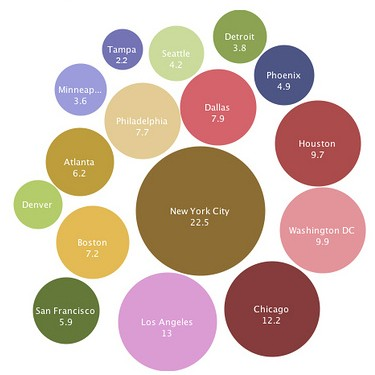
\includegraphics{img/time-cost.jpg}
\caption{\label{fig:fig1}Tempo de espera acumulado (em anos) por elevadores durante 12 meses em 16 cidades norte-americanas. Fonte:~\cite{IBM10}}
\end{figure}

Neste contexto global, a indústria de elevadores possui alguns desafios: primeiro, lidar com a pressão para a redução de custos na construção civil, construindo elevadores mais baratos e eficientes, com melhorias no desempenho de transporte; segundo, competir no mercado oferecendo serviços novos, personalizados e com garantia de qualidade, visando revolucionar a maneira com que elevadores interagem e servem passageiros~\cite{KOEHLEROTTIGER02}. Já sob o ponto de vista dos passageiros, estes esperam que suas chamadas sejam atendidas imediatamente e que sejam levados ao seu destino o mais rápido possível.

Existem diversas abordagens que os fabricantes de elevadores podem usar para minimizar o tempo de espera, como aumentar o número de elevadores no prédio ou a capacidade de cada elevador. Entretanto, este tipo de alteração não é sempre realizável em função de limitações na estrutura do prédio ou inviabilidade financeira. Como alternativa e muitas vezes uma solução de mais fácil aplicação é otimizar o sistema de controle dos elevadores. Ainda assim, a tarefa de atribuir elevadores para atender chamadas minimizando o tempo médio de espera está no conjunto de problemas NP-difícil (ou NP-hard, ou NP-complexo)~\cite{SeKo99}. Portanto, uma solução ótima para este problema ainda não é conhecida.

Desde meados dos anos 1980, a indústria de elevadores vem estudando e implementando estratégias para encontrar soluções sub-ótimas para o problema. Diversas técnicas de Inteligência Artificial foram adotadas, como redes neurais, algoritmos genéticos, lógicas \textit{fuzzy} e, mais recentemente, sistemas multi-agentes, planejamento e aprendizado de máquina~\cite{KOEHLEROTTIGER02}.

A proposta deste trabalho é comparar diferentes estratégias de controle de elevadores em alguns cenários e avaliar, dentre as opções possíveis, quais combinações resultam em um melhor desempenho no transporte de passageiros. A comparação se dará analisando os resultados de simulações de diferentes algoritmos de controle.

Para tanto, serão implementados no mínimo 2 algoritmos para o sistema de controle de elevadores e um simulador de elevadores. O usuário do simulador poderá:

\begin{itemize}
  \item Selecionar cenários;
  \item Selecionar um algoritmo para controle dos elevadores ou implementar o seu próprio;
  \item Comparar o desempenho entre diferentes algoritmos em um mesmo cenário;
  \item Comparar o desempenho de um algoritmo em múltiplos cenários.
\end{itemize}

\section{Métricas de Desempenho de um Sistema de Elevadores}


\begin{description}[leftmargin=!,labelwidth=\widthof{\bfseries HC\textsubscript{5\%}}]
  \item[HC\textsubscript{5\%}]
  Percentual da população total do prédio que um sistema de elevadores consegue transportar em um intervalo de 5 minutos. Um HC\textsubscript{5\%} aceitável é de no mínimo 14\% \cite{KOEHLEROTTIGER02}. Por exemplo, em um prédio cuja população é de 600 pessoas, este índice representa o transporte de no mínimo 84 pessoas em 5 minutos.

  \item[WT]
  \textit{Waiting Time}, ou tempo de espera; está compreendido entre a chegada de um passageiro e o seu embarque em um elevador.

  \item[JT]
  \textit{Journey Time}, ou tempo de jornada; está compreendido entre o embarque de um passageiro em um elevador e o desembarque em seu destino.

  \item[ST]
  \textit{System Time}, ou tempo de sistema; está compreendido entre entre a chegada de um passageiro e o desembarque em seu destino, ou seja, é a soma do tempo de espera com o tempo de jornada.

  \item[AWT]
  \textit{Average Waiting Time}, ou tempo médio de espera.

  \item[AJT]
  \textit{Average Journey Time}, ou tempo médio de jornada.


  \item[AST]
  \textit{Average System Time}, ou tempo médio de sistema.
\end{description}

O tempo médio de sistema define a qualidade do serviço, já que está ligada diretamente à percepção que os passageiros possuem do sistema. É correto afirmar que o desejo de um passageiro é chegar no seu destino o mais rápido possível - ou seja, com o menor tempo de sistema possível. Normalmente, tempos de sistema menores relacionam-se com um alto HC\textsubscript{5\%}; porém, passageiros tendem a dar maior importância a um baixo tempo de espera do que a um baixo tempo de jornada~\cite{KOEHLEROTTIGER02}.

 Ainda assim, embora não seja uma grande melhoria reduzir de 32 para 28 segundos de espera, é psicologicamente importante evitar esperas longas, i. e. 60 segundos ou mais. {\color{red}[BUSCAR FONTES PARA ESTA AFIRMAÇÃO]} % TODO: CITATIONNEEDED

 Assim sendo, o escopo deste trabalho será limitado na busca pela otimização do tempo médio de espera (\textbf{AWT}).

\section{Parâmetros de Definição de Cenários}

\begin{description}[leftmargin=!,labelwidth=\widthof{\bfseries AAA}]
  \item[F]
  Número total de andares do prédio.
  \item[E]
  Número total de elevadores que compõem o sistema.
  \item[K]
  Capacidade máxima de passageiros que um elevador é capaz de transportar.
  \item[P]
  População total do prédio.
  \item[F]
  Função de distribuição de chegada de passageiros.
\end{description}

\section{Glossário}

Termos chaves usados neste trabalho.

\begin{description}[leftmargin=!,labelwidth=\widthof{\bfseries Sistema de Controle}]
  \item[Lobby]                Andar térreo de um prédio.
  \item[Elevador]             Dispositivo de transporte vertical que movimenta pessoas ou cargas entre andares ou níveis de um prédio ou estrutura.
  \item[Sistema de Controle]  O sistema central que gerencia todos os elevadores.
\end{description}
\chapter{\label{chap:problem}Descrição do Problema}

A maior parte dos prédios possui instalações de grupos com 2 a 8 elevadores \cite{KOEHLEROTTIGER02}. Em muitos prédios, esses são o meio de transporte primário entre andares, visto que escadas são menos práticas e, muitas vezes, menos acessíveis ou exclusivas para situações de emergência. Dado o seu uso em larga escala, a ineficiência dos sistemas de controle de elevadores é sentida diariamente por seus usuários. Neste cenário, deseja-se encontrar formas de otimizar estes sistemas de controle de modo a refletir positivamente no desempenho geral do sistema e na percepção da qualidade do sistema na visão de seus usuários.

O problema estudado neste trabalho é modelado da seguinte forma: seja um prédio com \textbf{N} andares e \textbf{M} elevadores, cada um com capacidade para transportar \textbf{K} pessoas simultaneamente; sabe-se que a população total do prédio é \textbf{P} e está distribuída de maneira uniforme nos andares do prédio; também sabe-se que a chegada ou saídas destas pessoas obedece uma função de distribuição de probabilidade \textbf{F}. De que forma o sistema pode atender esta população de modo a minimizar o tempo médio de atendimento de cada pessoa?

\section{Sistema de Controle de Grupo de Elevadores}

Um \textit{Elevator Group Control System} (\textbf{EGCS}), ou sistema de controle de grupo de elevadores, é responsável por coordenar as ações dos elevadores do prédio~\cite{kuzunuki1984elevator}. Esta coordenação visa atender à todas \textbf{chamadas de corredor}\footnote{Passageiros estão fora dos elevadores e realizam uma chamada para subir ou descer à partir do andar em que se encontram.} e \textbf{chamadas de cabine}\footnote{Passageiros estão dentro do elevador e realizam uma chamada para desembarcar em um andar destino.} em um dado instante. O \textbf{estado} do sistema pode ser modelado, minimamente, pelo seguinte conjunto de informações:

\begin{itemize}
  \item Para cada andar:
  \begin{itemize}
    \item Se existe uma \textbf{chamada de corredor} a partir deste andar, o horário em que foi originada e o sentido (subir, descer ou ambos);
  \end{itemize}
  \item Para cada elevador:
  \begin{itemize}
    \item Um conjunto de \textbf{chamadas de cabine} solicitadas pelos passageiros e o horário em que cada uma foi originada;
    \item O andar em que se encontra;
    \item Se está parado, subindo ou descendo;
    \item Sua lotação.
  \end{itemize}
\end{itemize}

Sobre estes dados, o EGCS utiliza-se de algoritmos e técnicas para fornecer como saída:

\begin{itemize}
  \item Para cada elevador:
  \begin{itemize}
    \item Uma \textbf{sequência de paradas} que aquele elevador deve realizar.
  \end{itemize}
\end{itemize}

Existem eventos após os quais o EGCS deve recalcular as sequências de paradas dos elevadores de modo a atender as novas solicitações. Tais eventos são:

\begin{itemize}
  \item Uma nova \textbf{chamada de corredor};
  \item Uma nova \textbf{chamada de cabine};
  \item Uma \textbf{parada realizada} com alteração significativa na lotação do elevador;
  \item Um elevador torna-se ocioso, i. e., não possuir mais paradas a realizar.
\end{itemize}

\section{Aquisição de Dados e Métricas}

A aquisição de dados sobre o tráfego de um sistema de elevadores instalados é um problema em aberto na indústria~\cite{KOEHLEROTTIGER02}. Em casos simples é possível designar pessoas para observar e contar passageiros entrando e saindo dos elevadores. Já em casos mais complexos foram aplicadas soluções mais engenhosas, como contagem de pessoas aplicando algoritmos de visão computacional em vídeos de câmeras de segurança e sensores de carga. Estas abordagens possuem fatores complicadores - como, por exemplo, a dificuldade em lidar com as diferenças de iluminação, baixa qualidade de vídeo, baixa precisão de sensores, etc - e o resultado obtido não compensa o custo.

A simulação de sistemas de elevadores ganha destaque neste contexto, tornando-se uma alternativa atraente para obter métricas e avaliar o desempenho de um sistema na fase de projeto, antes da sua construção. Algumas das principais métricas utilizadas pela indústria de elevadores para avaliar o desempenho de seus sistemas são:

\begin{description}[leftmargin=!,labelwidth=\widthof{\bfseries HC\textsubscript{5\%}}]
  \item[HC\textsubscript{5\%}]
  Percentual da população total do prédio que um sistema de elevadores consegue transportar em um intervalo de 5 minutos. Um HC\textsubscript{5\%} aceitável é de no mínimo 14\%~\cite{KOEHLEROTTIGER02}. Por exemplo, em um prédio cuja população é de 600 pessoas, este índice representa o transporte de no mínimo 84 pessoas em 5 minutos.

  \item[WT]
  \textit{Waiting Time}, ou tempo de espera; está compreendido entre a requisição de um passageiro e o seu embarque em um elevador.

  \item[JT]
  \textit{Journey Time}, ou tempo de jornada; está compreendido entre o embarque de um passageiro em um elevador e o desembarque em seu destino.

  \item[ST]
  \textit{System Time}, ou tempo de sistema; está compreendido entre entre a chegada de um passageiro e o desembarque em seu destino, ou seja, é a soma do tempo de espera com o tempo de jornada.

  \item[AWT]
  \textit{Average Waiting Time}, ou tempo médio de espera.

  \item[AJT]
  \textit{Average Journey Time}, ou tempo médio de jornada.

  \item[AST]
  \textit{Average System Time}, ou tempo médio de sistema.

  \item[RTT]
  \textit{Round-trip Time}, ou tempo de ida e volta em uma tradução livre; é o tempo médio de uma viagem de um elevador partindo do lobby, indo até todos os andares do prédio e de volta ao lobby em horário de pico.
\end{description}

O tempo médio de sistema (AST) define a qualidade do serviço, já que está ligado diretamente à percepção que os passageiros possuem do sistema. É correto afirmar que o desejo de um passageiro é chegar no seu destino o mais rápido possível - ou seja, com o menor tempo de sistema possível. Normalmente, tempos de sistema menores relacionam-se com um alto HC\textsubscript{5\%}; porém, passageiros tendem a dar maior importância a um baixo tempo de espera do que a um baixo tempo de jornada~\cite{KOEHLEROTTIGER02}. Isto por que, uma vez dentro do elevador, o passageiro não se sente mais esperando: ele sente que já está sendo servido.

{\color{red}Ainda assim, embora uma redução de 32 para 28 segundos de espera não seja considerada uma grande melhoria, é psicologicamente importante evitar esperas longas, i.~e.~60 segundos ou mais.} % TODO: CITATIONNEEDED

\section{Padrões de Comportamento}

Há três padrões principais que descrevem o comportamento de grupos de
passageiros em relação aos elevadores.

\begin{description}[leftmargin=!,labelwidth=\widthof{\bfseries interfloor}]
  \item[up peak]    Passageiros chegam no lobby e desejam subir.
  \item[down peak]  Passageiros desejam descer de qualquer andar para o lobby.
  \item[interfloor] Passageiros deslocam-se entre andares arbitrários, com exceção do lobby.
\end{description}

Outros padrões podem ser definidos combinando-se os três padrões acima
descritos. No entanto, para os fins deste trabalho, nos limitaremos aos padrões puros.

\section{Cenários}

Pode-se dizer que cada prédio é um cenário em potencial no contexto deste trabalho. Alguns dos principais atributos que podem ser utilizados para definir um cenário são:

\begin{description}[leftmargin=!,labelwidth=\widthof{\bfseries Propósito}]
  \item[N]
  Número total de andares do prédio.
  \item[M]
  Número total de elevadores que compõem o sistema.
  \item[K]
  Capacidade\footnote{Como efeito de redução de escopo consideraremos todos os
    elevadores de um mesmo sistema como tendo a mesma capacidade.} (em número de
  pessoas\footnote{Consideramos uma pessoa com peso médio de 70kg.}) máxima de passageiros que cada elevador é capaz de transportar.
  \item[P]
  População total do prédio.
  \item[F]
  Função de distribuição de probabilidade de chegada/saída de passageiros.
  \item[Propósito]
  Propósito do prédio: residencial, comercial com múltiplas empresas, comercial com única empresa, etc;
\end{description}

Logo, há tantos cenários possíveis quanto há prédios ao redor do mundo.
Entretanto, por limitação de tempo e de recursos computacionais, vamos limitar
os cenários em algumas categorias. A escolha destas divisões é arbitrária, com
fim didático, exceto pelo limite inferior de 4 andares devido à exigência legal
do Município de Porto Alegre onde prédios deste tamanho ou maiores (mas não
menores que isto) de serem construídos com elevadores. O limite
superior\footnote{O maior arranha-céu do mundo em 2015 é o Burj Khalif,
  localizado em Dubai, com mais de 800m de altura, em 160 andares habitáveis.} fica em aberto.

% \footnote{http://www2.portoalegre.rs.gov.br/cgi-bin/nph-brs?u=/netahtml/sirel/avancada.html&p=3&r=59&f=G&d=ATOS&l=20&s1=(ELEVADOR)..RELA. }

\begin{table}[htb!]
\centering
\caption{Cenários}
\label{table:tab1}
\begin{tabular}{|l|c|c|c|c|}
\hline
{\bf Cenário}        & {\bf N}    & {\bf M} & {\bf K} & {\bf P} \\ \hline
{\it Prédio pequeno} & 4 a 5      & 1       & 6       & 40      \\ \hline
{\it Prédio médio}   & 6 a 10     & 2       & 10      & 96      \\ \hline
{\it Pŕedio grande}  & 11 a 30    & 5       & 10      & 560     \\ \hline
{\it Arranha-céu}    & 30 ou mais & 10      & 12      & 3200    \\ \hline
\end{tabular}
\end{table}

{\color{red}[SERIA BEM MELHOR SE USÁSSEMOS DADOS REAIS PARA MKP DE PRÉDIOS CONHECIDOS. EX: PŔEDIO ONDE MORAMOS, FACIN, EMPIRE STATE, BURJ KHALIF, ETC]} % TODO

\section{Critérios de Aceitação}

Uma tecnologia que saiba endereçar as seguintes questões será de grande interesse para a indústria de elevadores~\cite{KOEHLEROTTIGER02}:

\begin{enumerate}
\item Qual é a função objetivo de um algoritmo de despache em grupo? \hfill \newline
      Almost no information is published by companies about the objective functions they use in their con- trol algorithms. Usually, a vague “combination of waiting and journey times” is minimized, but which function would yield the best possi- ble results still seems to be an open question.

\item Como um sistema de controle pode obter informações adicionais acerca das necessidades dos passageiros?\hfill \newline
      In particular, how can it find out how many passengers are waiting at a floor, how fully loaded a car is, and where the passengers want to go?

\item Como o desempenho do controlador pode ser melhorado? \hfill \newline
      Is it possible to detect and predict patterns of traffic based on the cur- rently available information and/or previously learned patterns? How could such information be exploited by a control algorithm?

\item De quê forma as interfaces com os passageiros podem evoluir além de simples botões? \hfill \newline
      How can passengers with special needs be better served? In the following, we give an overview of AI- based approaches that have been explored by elevator companies in the past to address these issues.
\end{enumerate}

\section{Possíveis Complicadores}

Um número de cenários pode complicar as métricas e prejudicar os resultados. A grande maioria destes complicadores são fatores humanos, como pessoas segurando a porta, passageiros indecisos, seleção acidental de andares e desistências após chamar o elevador.

Alguns destes problemas podem ser mitigados com a modificação da interface dos elevadores. Por exemplo, seleções acidentais de andares poderiam ser desfeitas, caso houvesse um mecanismo para cancelar a seleção de um andar. O mesmo vale para o cenário do passageiro indeciso.

No entanto, propor este tipo de alteração de comportamento não está no escopo deste trabalho. É nosso objetivo estudar alterações somente nos algoritmos que regem o comportamento dos elevadores da maneira com que estão atualmente instalados na vasta maioria dos prédios.
\chapter{\label{chap:proposal}Proposta do Trabalho}

A proposta deste trabalho será estudar métodos de inteligência artificial,
aplicados a elevadores, de modo a aumentar a eficiência de grupos de elevadores.

As conseqüências imediatas esperadas deste aumento de eficiência são um ganho de
qualidade de vida para os potenciais passageiros, bem como um aumento de
produtividade de alguns grupos dos mesmos.

MODELAGEM

AGENTES

FUNÇÃO-OBJETIVO
\chapter{\label{chap:ai}Algoritmos de Inteligência Artificial para Elevadores}

Aqui vamos apresentar:

\begin{itemize}
\item Detalhar o(s) algoritmo(s) selecionados e justificar a sua escolha perante o problema;
\item Introduzir o modelo de simulação do sistema - ou seja, a modelagem do
prédio+andares+elevadores (e não a modelagem do simulador propriamente dito);
\item Apresentar em detalhe o algoritmo e descrever como esperamos que seja o resultado de seu uso junto ao sistema.
\end{itemize}

% TODO: Mais introdução
A literatura fala em alguns algoritmos utilizados para a escolha de qual
elevador atenderá um pedido. Alguns deles são triviais e não devem ser
enquadrados no termo Inteligência Artificial, no entanto, sua implementação é
interessante, no mínimo para fins de comparação com os demais algoritmos.
% TODO: Referências

\section{\label{sec:ai:nn}Nearest Neighbour}

O algoritmo de \textit{Nearest Neighbour} é o mais ingênuo de todos, e servirá
de base para a avaliação dos demais algoritmos.

Seu funcionamento é trivial: o elevador mais próximo do chamado sempre
atenderá este.

Um dos muitos problemas deste algoritmo é que ele pode causar muitas mudanças de
direção de um elevador, bem como um uso não justo dos elevadores, onde um
elevador fica maior parte do tempo parado.

% TODO: Quem fala nele?

\section{\label{sec:ai:nnm}Nearest Neighbour Melhorado}

Uma melhoria que pode ser feita ao algoritmo de \textit{Nearest Neighbour}
é considerar o sentido em que o elevador está indo para atender o chamado.

Este algoritmo resolve o problema de mudanças de direção que o algoritmo de
\textit{Nearest Neighbour} sofre, mas ainda pode resultar num uso pouco justo de
um elevador. % TODO: tirei isto do meu chapéu

No entanto, sua escolha para este trabalho também se dá para fim de comparação
com os outros e validação do simulador. Como seu comportamento é diferente do
caso mais trivial, mas ainda assim bastante simples, poderá ser visto com clareza
algum tipo de melhora no tempo de resposta do sistema, bem como a validade do simulador.

\section{\label{sec:ai:minimize-cost-function}Minimização da Função de Custo}

O primeiro algoritmo de IA a ser testado é simples: define-se uma
função de custo, que descreve matematicamente quão vantajoso é atender um
pedido, comparado a não atendê-lo. A decisão de qual elevador é escolhido para
atender o pedido é feita com base única e exclusivamente em qual deles terá o
menor valor da função de custo.

Várias funções de custo podem ser experimentadas e comparadas.

Um exemplo de função de custo é:

\[
  J(f) = \sum_{i=0}^{i=n} g_{i}f
\]

Onde $g_{i}$ é cada grupo no sistema e $f$ é a distância, em número de andares,
entre a posição atual do elevador e o pedido que se está avaliando.

Outras funções de custo levariam em consideração mudanças de direção de viagem
\footnote{\textit{e.g.}, pode ser vantajoso um elevador mudar de direção para atender um
pedido a um andar de distância, caso a alternativa seja fazer o pedido esperar
um deslocamendo de dezenas de andares de outro elevador.}, ou ainda tentar
manter todos os custos o mais baixo possível, ao mesmo tempo que sejam todos o
mais próximos uns dos outros.\footnote{É possível elevar cada termo do somatório ao
  quadrado para obter-se isto.}

% TODO: outros exemplos de função de custo?

\section{Planning}

% TODO: essa explicação pode melhorar ainda

A idéia do algoritmo de planning é estender o de função de custo, calculando a
mesma para vários passos no futuro~-~como em um jogo de xadrez.

O horizonte de cálculo deve ser selecionado, dado que é um fator limitante no
tamanho do cálculo do algoritmo.

Cada decisão diferente, para cada elevador, é um nodo novo na árvore. Ao
escolher-se uma das alternativas (\textit{i.e.} a que, ao final de $x$ eventos
no futuro tem o menor custo), avança-se um passo na simulação e executa-se o
algoritmo novamente.

Na Figura~\ref{fig:planning}, vemos um exemplo de planning sendo executado com
horizonte 3 e dois elevadores. Para cada passo do algoritmo, a decisão a ser
tomada é ``qual elevador deve atender o próximo pedido da fila?'', e, para isto,
calcula-se a função de custo. O resultado da função pode ser visto entre
parênteses em cada nodo da árvore da Figura~\ref{fig:planning}.

Ao encontrarmos o horizonte (no caso da Figura~\ref{fig:planning}, no nível 3 da
árvore), vemos quem tem o menor custo (neste caso, E2, filho de E2, filho de
E1). Toma-se então a decisão de descer um nível na árvore apenas, em direção ao
menor custo.

Veja que, ao fazer isto, poderá tomar-se uma decisão diferente do algoritmo que apenas
considera a função de custo. No caso da Figura~\ref{fig:planning}, o elevador E1
atenderá o próximo chamado, mesmo tendo um custo superior a E2.

\begin{figure}[htb!]
  \centering
  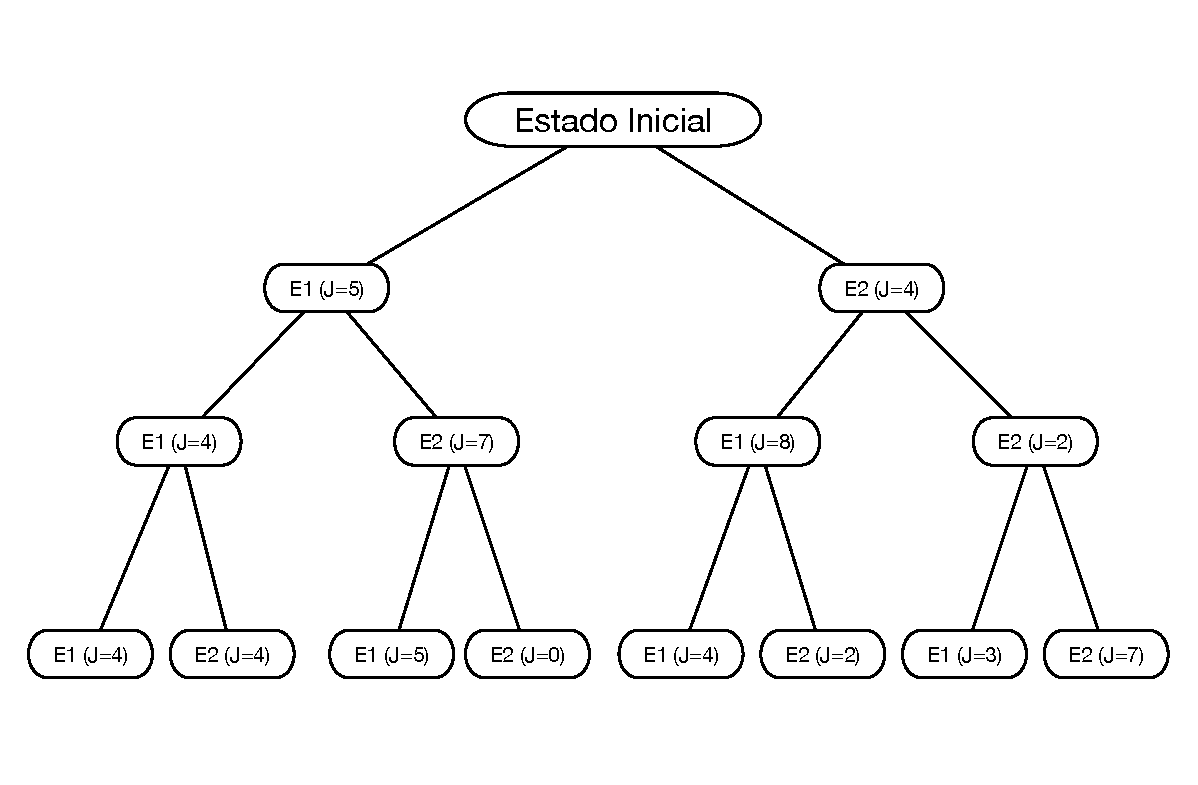
\includegraphics[scale=0.8]{img/planning.eps}
  \caption{Exemplo de planning com horizonte 3 e dois elevadores}
\label{fig:planning}
\end{figure}

\section{Planning Multi-Agente}

Este algoritmo é uma extensão do algoritmo de Planning, onde, em vez de termos
um processamento central que decide que um elevador deve atender o pedido, temos
todos os elevadores calculando por conta própria se vale a pena atender um
pedido ou não~-~sem conhecimento do estado dos demais.

A literatura neste tópico é bastante escassa ainda.
\chapter{\label{chap:simulation}Sistemas e Simulações}

``Simulação é a imitação da operação de um sistema ou processo do mundo real ao
longo do tempo.'' \cite{Banks}. Em outras palavras, simulação envolve a geração
de uma história artificial de um sistema ou processo e a observação desta
história de modo a obter inferências a respeito das características operacionais
da realidade ali representada.

A fim de estudar um sistema, frequentemente existe a necessidade de realizar uma
série de suposições sobre como ele funciona. Estas suposições, que normalmente
assumem a forma de relações matemáticas ou lógicas, constituem um modelo que é
utilizado para se tentar obter algum entendimento sobre como o sistema
correspondente se comporta.

\section{Quando Simulação Não é Indicada}

Para estudar e compreender um sistema e suas características, existem diversas
abordagens - dentre elas a simulação. Entretanto, é de suma importância que cada
sistema seja analisado com a melhor ferramenta em cada caso. Existe uma
infinidade de sistemas onde a simulação não é a forma apropriada para estudo.
\cite{BanksGibson} define 10 situações onde a simulação \textbf{não} é indicada:

\begin{enumerate}
\item Quando o problema puder ser resolvido utilizando-se de bom senso;
\item Quando o problema puder ser resolvido de forma analítica;
\item Quando o problema puder ser resolvido através de experimentos diretamente
      no sistema;
\item Quando seus custos da simulação excederem os seus ganhos;
\item Quando não há recursos financeiros suficientes;
\item Quando não há tempo suficiente;
\item Quando não há dados suficientes, nem mesmo estimativas;
\item Quando não há possibilidade de verificar a validade do modelo;
\item Quando as expectativas e o poder da simulação são superestimados - ou
      seja, \textbf{simulação não é bala de prata};
\item Quando o comportamento do sistema é muito complexo ou não pode ser
      definido (e.~g. seres humanos).
\end{enumerate}

\section{Formas de Estudar um Sistema}

Por outro lado, \cite{Law} oferece 3 perguntas para decidir qual a melhor forma
de se estudar um sistema específico (figura \ref{fig:systemstudy}). São elas:

\begin{figure}[htb!]
\centering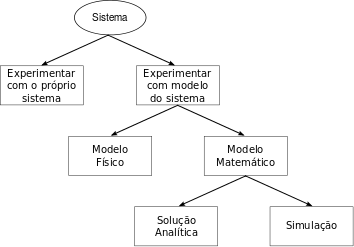
\includegraphics{img/systemstudy.png}
\caption{\label{fig:systemstudy}Formas de estudar um sistema. Fonte:~\cite{Law}}
\end{figure}

\begin{enumerate}
\item Experimentar com o próprio sistema ou experimentar com um modelo do mesmo?

Se houver viabilidade técnica e financeira na alteração de um sistema e na
observação de sua operação sob as novas condições, é desejável que se faça as
experimentações com o próprio sistema. Entretanto, frequentemente esta
alternativa é inviável por diversas razões:

\begin{itemize}
  \item O custo dos experimentos é muito elevado:

  % TODO - indentar no texto
  Exemplo: construir um novo módulo na Estação Espacial Internacional.

  \item O impacto causado pelos experimentos pode ser prejudicial ao sistema:

  % TODO - indentar no texto
  Exemplo: um mercado deseja reduzir o número de caixas a fim de diminuir seus
custos operacionais. Porém, esta medida pode causar um aumento significativo no
tamanho das filas - e consequentemente uma piora no tempo de espera dos clientes
e causar desistências.

  \item O sistema não existe:

  % TODO - indentar no texto
  Exemplo: o sistema ainda está nas fases de \textit{inception}, projeto ou
  desenvolvimento.
\end{itemize}

Por isto, muitas vezes é necessário realizar os experimentos utilizando um
\textit{modelo} como substituto ao sistema real.

\item Experimentar utilizando um modelo físico do sistema ou utilizar um modelo
matemático?

Cockpits de aviões desacoplados do resto da nave, automóveis em escala em túneis
de vento e miniaturas funcioneis de sistemas de elevadores são alguns exemplos
de modelos físicos de sistemas. Ocasionalmente, este tipo de modelo é utilizado
é utilizado para estudar sistemas de engenharia ou logística \cite{Law}.
Entretanto, a vasta maioria de modelos são matemáticos, representando um sistema
em termos de relações lógicas e quantitativas (equações matemáticas e notações
simbólicas), que são então manipuladas e alteradas para observar de que forma o
sistema real reagiria - isto se o modelo matemático for válido.

\item O problema pode ser resolvido de forma analítica?

De posse de um modelo matemático, o mesmo deve ser examinado de modo a verificar
de qual modo ele pode ser utilizado para dar solução ao problema que ele
representa. Segundo \cite{Law}, se o modelo for simples o suficiente,
possivelmente é possível trabalhar com suas relações e equações para obter uma
solução exata, anaĺitica. \cite{Law} cita como exemplo o modelo $d = vt$, onde
$d$ é a distância, $v$ é a velocidade média e $t$ é o tempo de viagem. Se
soubermos a distância a ser viajada e a velocidade, podemos trabalhar no modelo
e encontrar a equação $t = d/r$ para encontrar, exatamente, o tempo de viagem.
Embora esta solução seja simples, não é incomum a busca por soluções analíticas
tornar-se extraordinariamente complexa, exigindo vastos recursos computacionais.

Portanto, se uma solução analítica para um problema é conhecida e possui
eficiência computacional, é mais apropriado estudar este sistema desta forma do
que através de simulação. Do contrário, o sistema deve ser estudado através de
simulações - ou seja, exercitar numericamente as entradas do modelo matemático
do sistema e observar de que forma estes exercícios afetam as saídas.
\end{enumerate}

\subsection{Formas de Estudar um \textit{Elevator Group Control System}}

De modo a justificar a escolha pelo uso da simulação ao estudar um
\textit{Elevator Group Control System}, as perguntas feitas na seção anterior
são respondidas:

\begin{enumerate}
\item Experimentar com o próprio sistema ou experimentar com um modelo do mesmo?

Entre os recursos de pesquisa deste trabalho não está disponível um sistema de
elevadores instalado para realizar as experimentações. Logo, optou-se pela
utilização de um modelo.

\item Experimentar utilizando um modelo físico do sistema ou utilizar um modelo
matemático?

Um modelo físico de um sistema de elevadores poderia ser constituído pela
maquete de um prédio, mini-elevadores movidos por motores de passo que por sua
vez seriam controlados por microcontroladores. Entretanto, este projeto por si
só já seria grandioso demais - além de, obviamente, fugir do escopo da Ciência
da Computação e ser mais adequado à um trabalho de conclusão de Engenharia
Elétrica ou Engenharia de Controle e Automação. Além disso, os experimentos
estariam limitados pelo número de andares e elevadores da maquete. Portanto,
optou-se por um modelo matemático do sistema, reproduzível em ambiente
computacional e facilmente parametrizável para diferentes cenários.

\item O problema pode ser resolvido de forma analítica?

Dada a complexidade de situações possíveis em um sistema de elevadores e os
esforços da indústria em procurar soluções engenhosas para resolver o problema,
pode-se inferir que não existe uma solução analítica conhecida para este
problema. Portanto, a simulação é uma alternativa indicada para o estudo de
problemas desta natureza.

\end{enumerate}

\section{Classificação do Modelo de Simulação}

Portanto, dado um modelo matemático a ser estudado por meio de simulação
(doravante chamado de modelo de simulação), o mesmo pode ser classificado em
três dimensões \cite{Banks,Law}:

\begin{enumerate}
\item Estático ou Dinâmico

Um modelo de simulação estático é uma representação de um sistema em um ponto
particular no tempo, ou então um modelo que represente um sistema onde o tempo
simplesmente é irrelevante. Por outro lado, um modelo de simulação dinâmico
representa um sistema que evolui e se modifica com o passar do tempo.

\item Determinístico ou Estocástico

Muitas vezes, bla bla bla.

\item Contínuo ou Discreto

Muitas vezes, bla bla bla.

\end{enumerate}
\chapter{\label{chap:modeling}Modelagem do Sistema}

Conforme visto final do \ref{chap:simulation}, um sistema de simulação possui
uma série responsabilidades bem definidas. Neste estudo o sistema será projetado
através das construções do paradigma da orientação à objetos. A opção pela
Orientação à Objetos se dá por diversos motivos:

\begin{itemize}
  \item encapsulamento
  \item abstração
  \item padrão de mercado
  \item padrão acadêmico
\end{itemize}

\section{Eventos e Tipos de Eventos}

O simulador é orientado à eventos. Logo, é necessário ter uma representação de
um evento na implementação. Um evento deve possuir as seguintes informações:
tipo de evento; horário em que o evento está agendado; um cliente (passageiro)
e/ou um elevador e/ou um andar do prédio\footnote{A existência de informações
sobre o cliente, o elevador e o andar dependem do tipo de evento.}. Já os tipos
de eventos possíveis são:

\begin{description}
  \item[Chegada de um cliente] um cliente chegou na fila de um andar;
  \item[Chegada de um elevador] um elevador chegou a um andar;
  \item[Elevador moveu-se para cima] um elevador moveu-se para cima;
  \item[Elevador moveu-se para baixo] um elevador moveu-se para baixo.
\end{description}

A figura \ref{fig:diagram:event} exibe o diagrama UML da classe \textit{Event} e
a enumeração \textit{EventType}.

\begin{figure}[htb!]
  \centering
  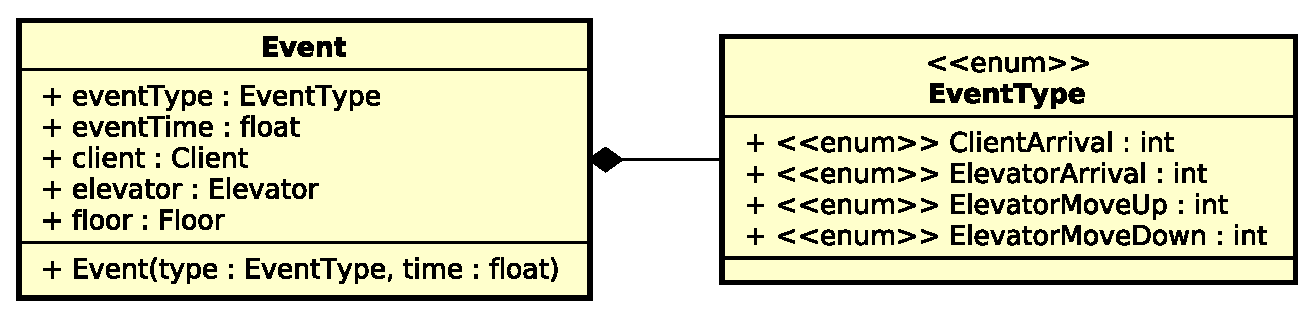
\includegraphics[scale=0.6]{img/event.eps}
  \caption{Classes para Eventos e Tipos de Eventos}
\label{fig:diagram:event}
\end{figure}

\section{Notificando Eventos}

Em um simulador, há a necessidade de executar diferentes ações na ocasião de um
evento específico. Por exemplo, atualizar o estado atual do sistema, as
estatísticas e o relógio da simulação. De acordo com Gamma
\cite{Gamma:1995:DPE:186897}, um \textit{design pattern} da programação
Orientada à Objetos indicado para o problema de notificar componentes que um
determinado evento ocorrereu é chamado de \textit{Observer}. Este
\textit{pattern} define uma dependência de um-para-muitos entre objetos de modo
que, quando este um objeto tem seu estado alterado, todos os seus dependentes
são notificados automaticamente. Por consequencia, estes objetos podem modificar
seu estado interno baseando-se nas informações desta notificação.

A figura \ref{fig:diagram:notification} ilustra as classes projetadas deste
sistema de Notificação de Eventos. A interface \textit{EventObserver} deve ser
realizada por qualquer classe que deseje receber eventos. Já a interface
\textit{EventNotifier} define a interface pública de um notificador de eventos.
Esta interface provê métodos que objetos \textit{EventObserver} possam se
registrar ou desregistrar para receber notificações das ocorrências de um
determinado tipo de evento, além de um método para realizar a notificação
propriamente dita do evento.

\begin{figure}[htb!]
  \centering
  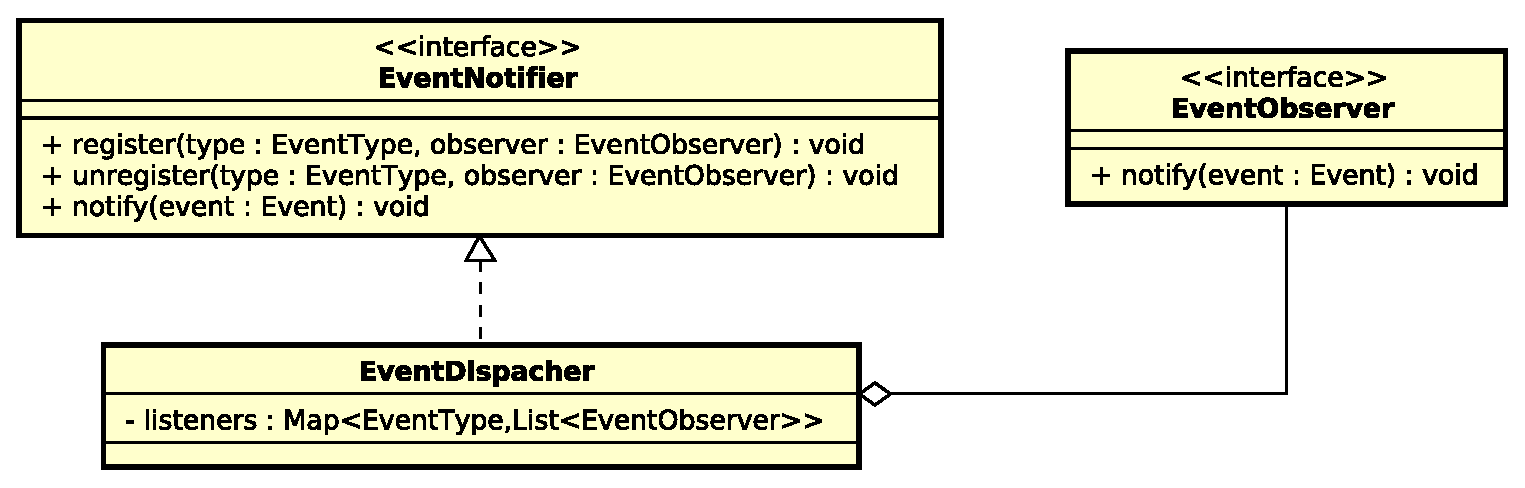
\includegraphics[scale=0.6]{img/notification.eps}
  \caption{Diagrama de Classes do Notificador de Eventos}
\label{fig:diagram:notification}
\end{figure}

A classe concreta \textit{EventDispatcher} realiza a interface
\textit{EventNotifier}. Para armazenar os objetos que deverão receber
notificações para cada evento, é utilizado um mapa que relaciona tipo de evento
com uma lista de \textit{EventObservers}. Na ocasião da ocorrência de um evento,
o \textit{EventDispatcher} é responsável por varrer a sua lista interna de
assinantes e notificá-los conforme o tipo de evento ocorrido.

Esta construção é bastante útil no momento em que possuímos três importantes
componentes do sistema que necessitam alterar o seu estado interno a cada evento
ocorrido (figura \ref{fig:diagram:observers}). São eles: \textit{Timer},
responsável por encapsular o relógio da simulação; \textit{Statistics},
responsável pela acumulação das estatísticas da simulação; e \textit{Building},
entidade que armazena o estado do prédio em si, com seus andares, elevadores e
passageiros. Na ocorrência de um evento, estas três entidades devem ser
notificadas e cada uma irá alterar seu estado interno da forma que lhe convir.

\begin{figure}[htb!]
  \centering
  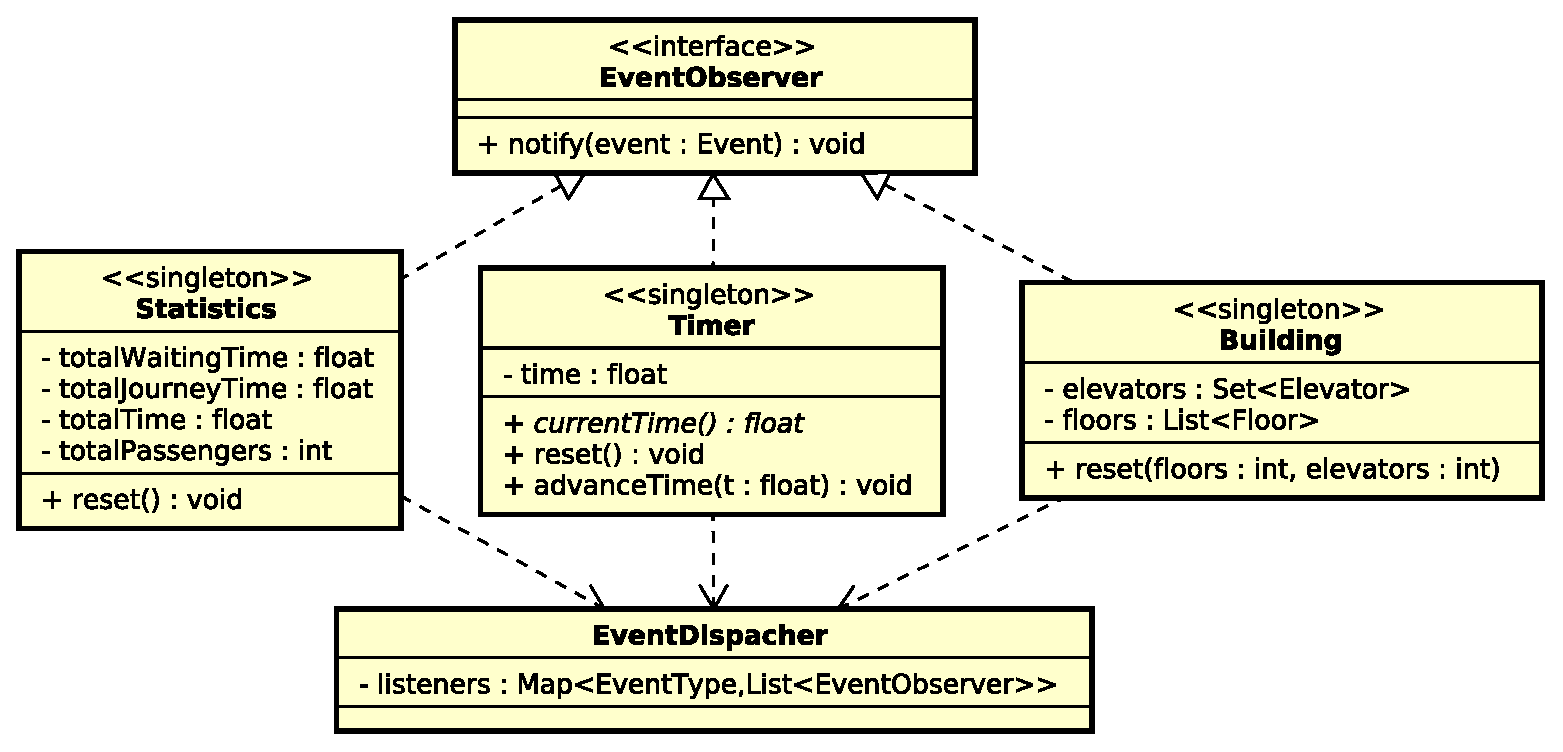
\includegraphics[scale=0.6]{img/observers.eps}
  \caption{Diagrama de Classes dos Observadores de Eventos}
\label{fig:diagram:observers}
\end{figure}

\begin{figure}[htb!]
  \centering
  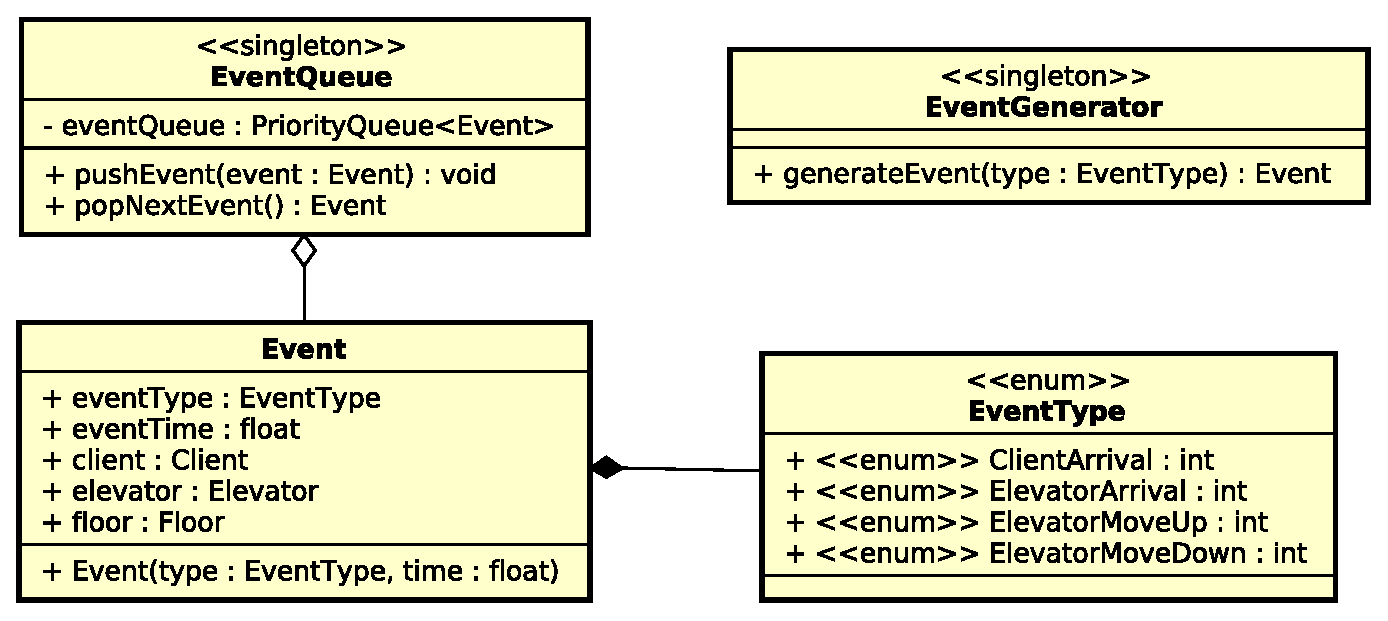
\includegraphics[scale=0.6]{img/event_management.eps}
  \caption{Diagrama de Classes do Gerenciador de Eventos}
\label{fig:diagram:event:manage}
\end{figure}

\begin{figure}[htb!]
  \centering
  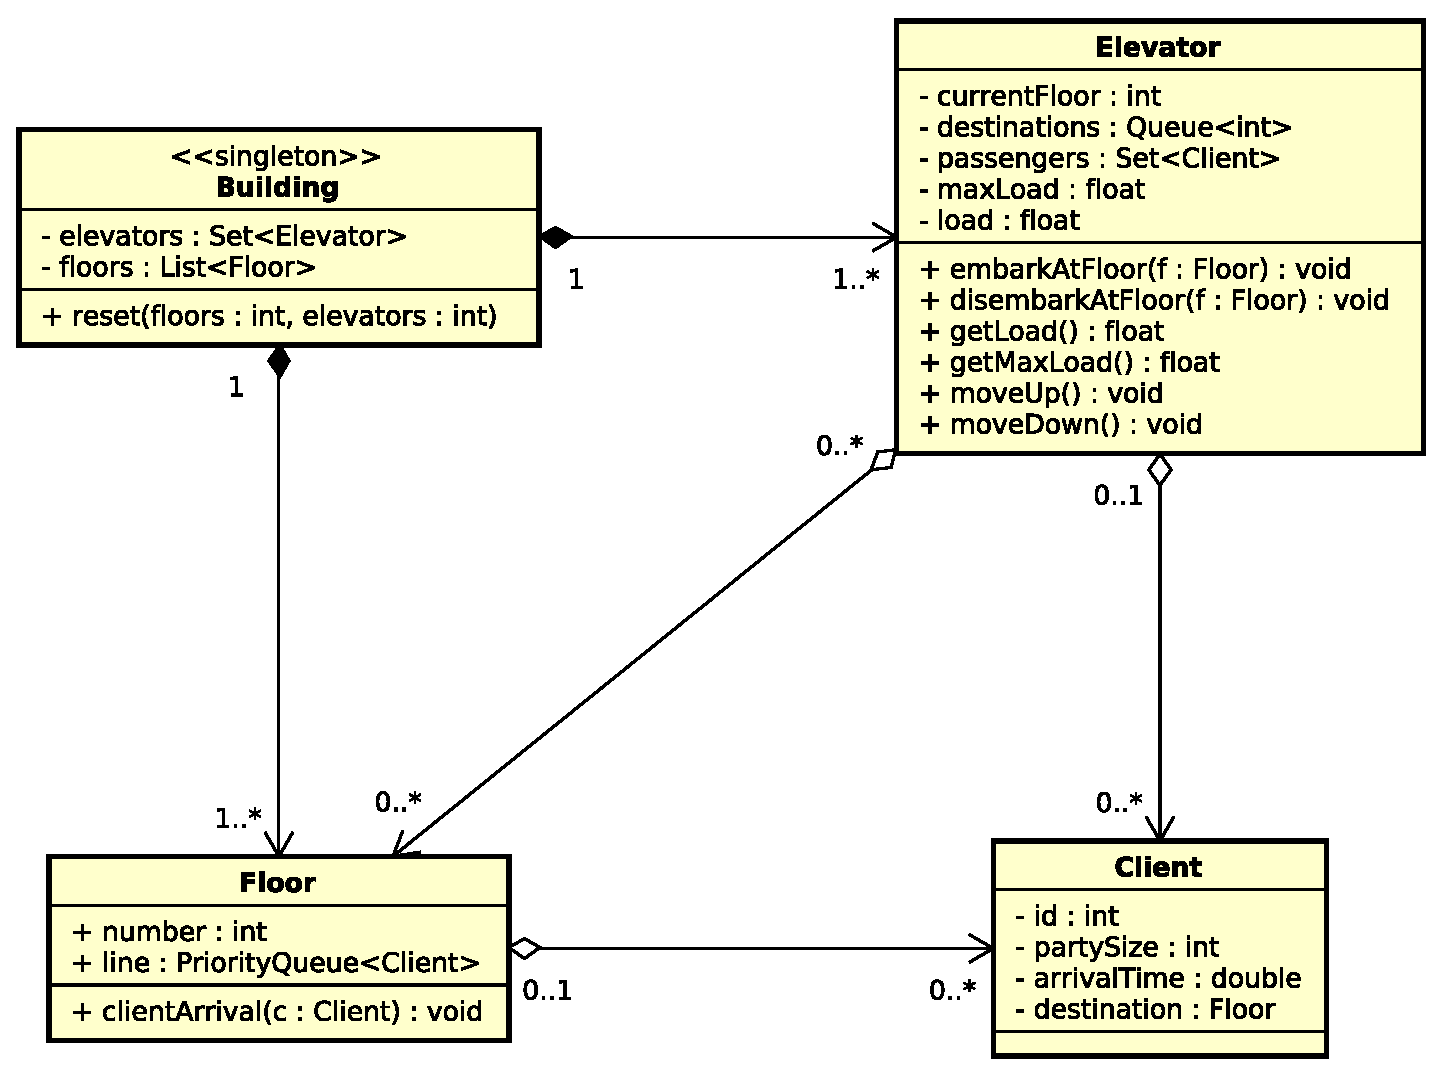
\includegraphics[scale=0.6]{img/state.eps}
  \caption{Diagrama de Classes da Representação do Estado do Sistema}
\label{fig:diagram:system}
\end{figure}

\begin{figure}[htb!]
  \centering
  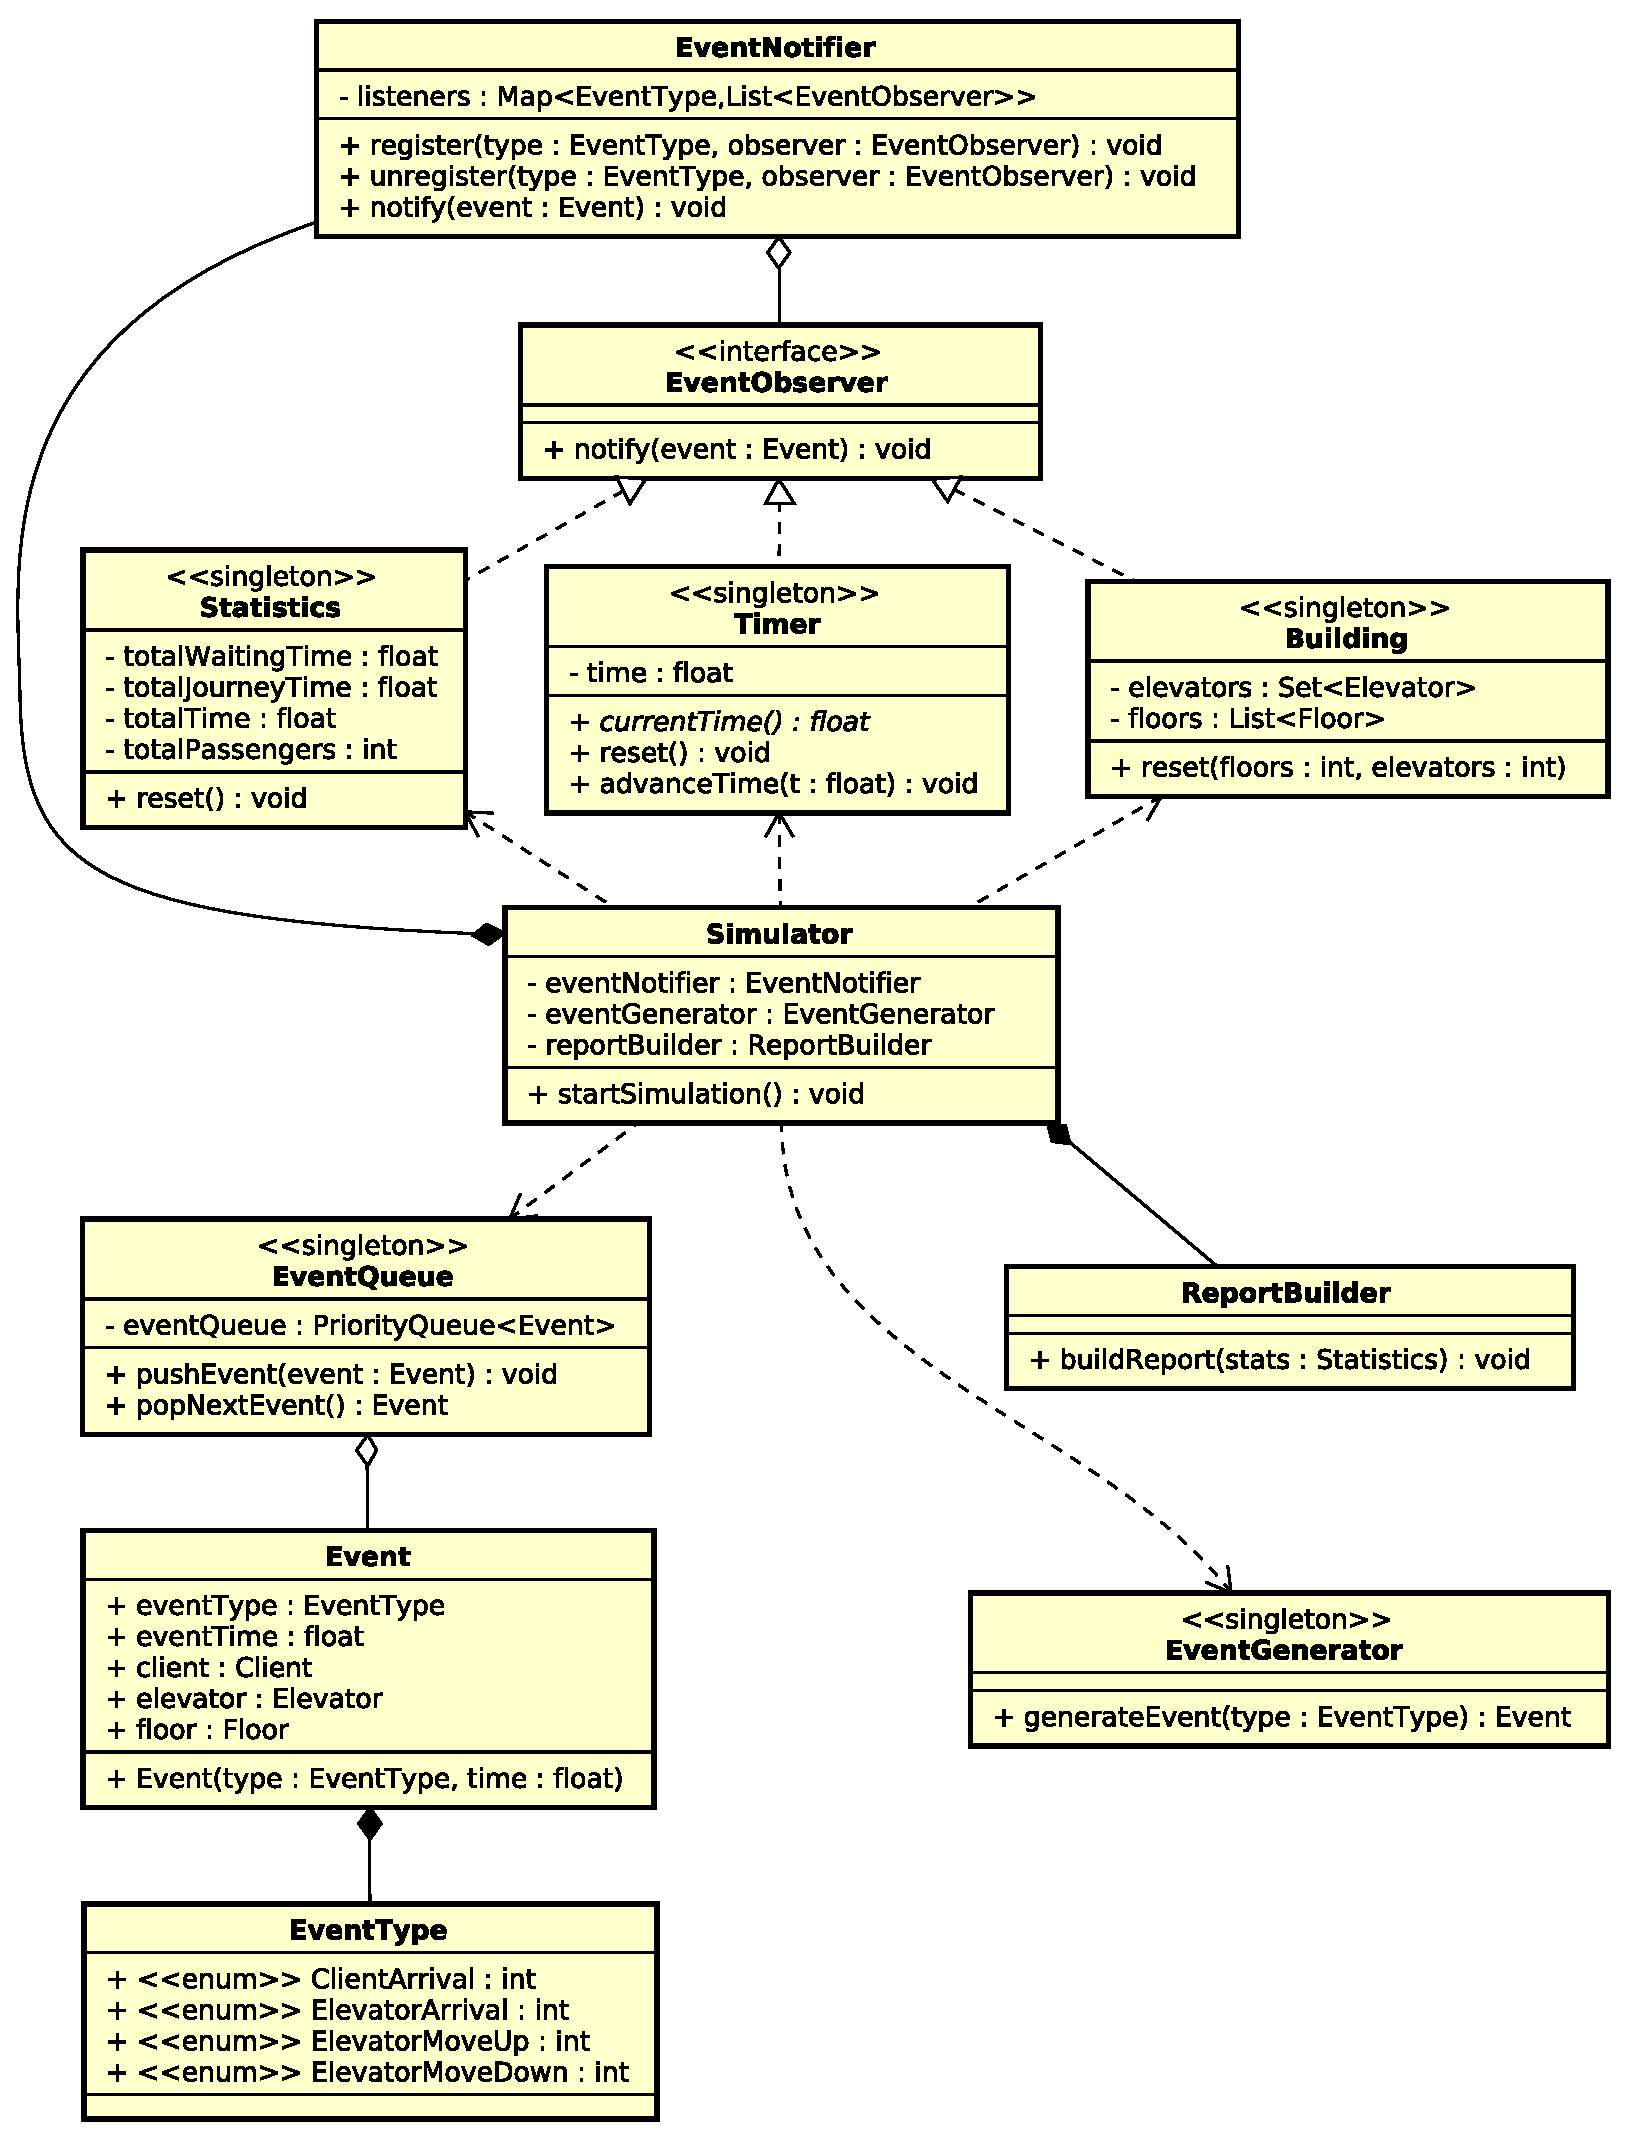
\includegraphics[scale=0.6]{img/simulator.eps}
  \caption{Diagrama de Classes do Simulador}
\label{fig:diagram:simulator}
\end{figure}


\subsection{aaaaaaaa}

Aqui vamos apresentar:

\begin{itemize}
  \item Descrições e diagramas UML dos componentes (classes, algoritmos, etc)
que dão sentido à simulação - ou seja, o modelo do sistema de elevadores
  \item Algoritmos e fluxogramas dos eventos do simulador que causarão
alterações no estado do sistema quais informações desejamos que o simulador
calcule para nós.
\end{itemize}

\section{\label{chap:input}Entrada de Distribuição de Probabilidade}

Aqui vamos apresentar:

\begin{itemize}
\item Conceitos sobre distribuições de probabilidade;
\item Conceitos sobre geração de variáveis aleatórias em ambiente computacional;
\item Descrever o modelo selecionado de processo de chegada de clientes
(passageiros);
\item Algoritmos e fluxogramas dos eventos do simulador que causarão alterações
no estado do sistema.
\end{itemize}
\chapter{\label{chap:related}Trabalhos Relacionados}

Alguns trabalhos já abordaram a temática de Inteligência Artificial aplicada a
elevadores. O artigo ``\textit{An AI-based approac to destination control in
  elevators}''~\cite{KOEHLEROTTIGER02} descreve o problema e o classifica como
NP-Hard.  %TODO CONTINUAR




\section{Destination Dispatch}

%http://www.schindler.com/br/internet/pt/solucoes-em-mobilidade/produtos/gerenciamento-acesso/miconic-10.html

Rockefeller Center, New York NY
Prime Tower, Zurich, Switzerland (2011)

%http://www.schindler.com/br/internet/pt/solucoes-em-mobilidade/produtos/gerenciamento-acesso/port-technology.html

EZ Towers
São Paulo, 2012

Doha Twin Towers
Doha, 2013

%https://www.thyssenkruppelevator.com/elevator-products/elevator-destination-dispatch#tab1

World Financial Center, NY, EUA

\section{Double-deck Elevators}

%http://www.schindler.com/content/au/internet/en/mobility-solutions/products/elevators/schindler-7000/_jcr_content/rightPar/downloadlist_0/downloadList/16_1336648631250.download.asset.16_1336648631250/DD_Brochure.pdf

Utilizado em:

Burj Khalifa in Dubai
Petronas Twin Towers in Kuala Lumpur
Statue of Liberty in New York (goes no higher than the pedestal)

\section{Two elevators, same shaft}

https://twin.thyssenkrupp-elevator.com/

Utilizado em:

European Central Bank, Frankfurt, Alemanha
ThyssenKrupp Headquarters, Essen, Alemanha
Mercury Tower Lot 14, Moscou, Russie
\chapter{\label{chap:conclusion}Conclusão}

Com elevadores presentes na vida de tantos habitantes de grandes centros
urbanos, eles são um alvo óbvio para otimização.

Como vimos anteriormente, algumas tentativas de utilização de Inteligência
Artificial aplicadas aos mesmos foram feitas. Entende-se que um simulador que
permita a avaliação objetiva e comparação de diferentes estratégias em
diferentes cenários será de grande valor, permitindo que decisões a respeito da
otimização e melhoria deste meio de transporte sejam tomadas.

A análise cuidadosa dos dados estatísticos gerados por este simulador permitirá
que uma estratégia vantajosa seja encontrada para cada cenário.

\bibliographystyle{tcc-num}
\bibliography{bib-proposta}

\end{document}
